\documentclass{book}

\usepackage{graphicx}
\usepackage{xcolor}
\usepackage{sectsty}
\definecolor{ChapterBlue}{rgb}{0.1,0.6, 0.9}
\chapterfont{\color{ChapterBlue}}  % sets colour of chapters
\sectionfont{\color{cyan}}


\usepackage[german]{babel}
\pagestyle{plain}
\title{Design Document}
\author{Christian Stricker \and David Klopp \and Markus Vieth}
\date{\today}

\begin{document}


Um zu verstehen wie die Interaktion zwischen Nutzer und System funktioniert, ist es notwendig die Kommunikation der einzelnen Komponenten, die zuständig zum Generieren des UI sind, näher zu beleuchten. 
Besonders geeignet hierfür ist das Model-View-Controller (MVC) Pattern. 
Im folgenden wird zunächst genauer auf die Erzeugen der UI, in unserem Fall eine Website, und anschließend auf die Einbindung einzelner Darstellungskomponenten in dieses eingegangen. \\

\begin{center}
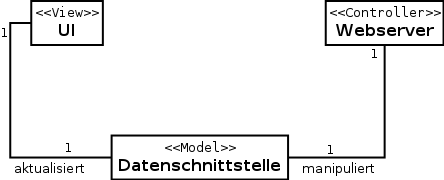
\includegraphics[scale=0.6]{../Grafik/Diagramm/Pattern/MVC/Website/Kontextdiagramm.png}
\end{center}

Die Website ist der für den Benutzer sichtbare Teil des Systems. Betätigt der Nutzer auf dieser Seite eine Schaltfläche, so werden seine Eingaben durch den Webserver ausgewertet und an die entsprechenden Instanzen im System weitergeleitet. Sollen in etwa benutzerbezogene Daten abgefragt werden, so greift der Webserver auf die Datenschnittstelle zu, die die entsprechenden Daten über eine SPARQL Anfragen an die RDF-Datenbank bereitstellt. Auf Basis dieser Rückgabe generiert der Webserver nun die entsprechende Website und  zeigt sie dem Nutzer an.
Sollten sich die Daten in der Datenbank ändern, so registriert die Datenschnittstelle dies und informiert die Website entsprechend, damit die Anzeige geupdated werden kann.

\begin{center}
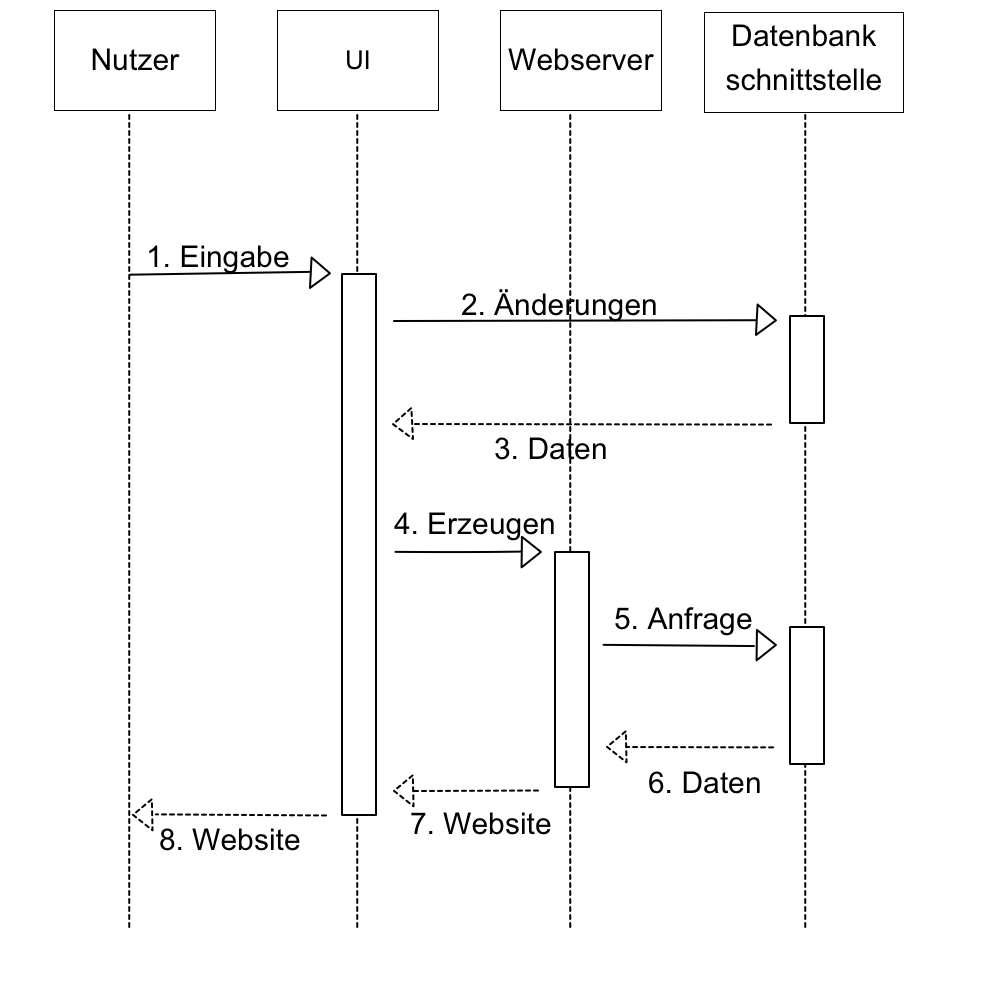
\includegraphics[width=1.0\linewidth]{../Grafik/Diagramm/Pattern/MVC/Website/Sequenzdiagramm.png}
\end{center}

\end{document}